\documentclass[12pt]{article}
\usepackage{amsmath}
\usepackage{graphicx}

%\setlength\parindent{20pt} %% Do not touch this

\title{Homework 1} 

\author{Geneva Porter\\ 
MATH-693B Numerical Partial DIfferential Equations\\}

\date{February 10, 2020} 
\begin{document}
\maketitle

\section*{1.1.1}

Consider the initial value problem for the equation
$$
u_{t}+a u_{x}=f(t, x)
$$
$$
\text { with } u(0, x)=0 \text { and } \quad f(t, x)=\left\{\begin{array}{ll}
{1} & {\text { if } x \geq 0} \\
{0} & {\text { otherwise }}
\end{array}\right.
$$
Assume that $a$ is positive. Show that the solution is given by
$$
u(t, x)=\left\{\begin{array}{ll}
{0} & {\text { if } x \leq 0} \\
{x / a} & {\text { if } x \geq 0 \text { and } x-a t \leq 0} \\
{t} & {\text { if } x \geq 0 \text { and } x-a t \geq 0}
\end{array}\right.
$$

\subsubsection*{Solution}

When $f(t,x)=0$, we have the unique solution $u(t,x) = u_0(x-at)$. This gives the answer $u_0(x-at) = u(0, x-at) = 0$, which is the indicated solution for all $x<0$. 

For $f(t,x)=1$ and $x-at <0$, we can show that the solution $u(t,x)=x/a$ is valid. Observe:


\begin{equation*}
\begin{aligned}
u(t,x) = \frac{x}{a} ~~~ \longrightarrow ~~~ u_t = 0 ~~~ \text{and} ~~~ u_x = \frac{1}{a}
\end{aligned}
\end{equation*}

\noindent Plugging this into our problem, we see that the result is $0 +a(1/a) = 1$, which is true. So this solution is correct.

For $f(t,x)=1$ and $x-at \geq 0$, let's change variables so that

$$ \tau=t ~~~~~\text{and} ~~~~~ \xi=x-at ~~~ \longrightarrow ~~~ x = \xi +a\tau.$$

\noindent Now we have $\tilde{u}(\tau, \xi) = u(t,x)$, and it follows that

\begin{equation*}
\begin{aligned}
	 \frac{\partial\tilde{u}}{\partial\tau} &= \frac{\partial t}{\partial\tau}u_t + \frac{\partial x}{\partial\tau}u_x\\
	 &= u_t + au_x = f(\tau, \xi+a\tau).
\end{aligned}
\end{equation*}

\noindent With $\frac{\partial\tilde{u}}{\partial\tau}=f(\tau, \xi+a\tau)$, we can solve this as an ordinary differential equation, which has the following solution:

\begin{equation*}
\begin{aligned}
	\tilde{u}(\tau,\xi)& = u_0(\xi) + \int_0^\tau f(\sigma, \xi+a\sigma) d\sigma ~~~ \longrightarrow \\
	u(t,x) &= u_0(x-at) + \int_0^t f(s,x-a(t-s)) ds\\
	&= 0 + \int_0^t ds = \left.\frac{}{}s\right|_0^t = t
\end{aligned}
\end{equation*}

And we see that this is indeed the solution we were seeking.




\section*{1.3.1}

For values of $x$ in the interval $[-1,3]$ and $t$ in $[0,2.4],$ solve the one-way wave equation $u_{t}+u_{x}=0$ with the initial data
$$u(0, x)=\left\{\begin{array}{ll}
{\cos ^{2} \pi x} & {\text { if }|x| \leq \frac{1}{2}} \\
{0} & {\text { otherwise }}
\end{array}\right.$$
and the boundary data $u(t,-1)=0.$
Use the following four schemes for $h=1 / 10,~1 / 20,$ and $1 / 40$:
\begin{enumerate}
	\item
	\begin{enumerate}
		\item Forward-time backward-space scheme $(1.3 .2)$ with $\lambda=0.8$
		\item Forward-time central-space scheme $(1.3 .3)$ with $\lambda=0.8$
		\item Lax-Friedrichs scheme $(1.3 .5)$ with $\lambda=0.8$ and 1.6
		\item Leapfrog scheme $(1.3 .4)$ with $\lambda=0.8$.
	\end{enumerate}
\end{enumerate}



For schemes (b). (c), and (d), at the right boundary use the condition $v_{M}^{n+1}=$ $v_{M-1}^{n+1},$ where $x_{M}=3 .$ For scheme (d) use scheme (b) to compute the solution at $n=1$
For each scheme determine whether the scheme is a useful or useless scheme. For the purposes of this exercise only, a scheme will be useless if $\left|v_{m}^{n}\right|$ is greater than
5 for any value of $m$ and $n .$ It will be regarded as a useful scheme if the solution looks like a reasonable approximation to the solution of the differential equations. Graph or plot several solutions at the last time they were computed. What do you notice about the "blow-up time" for the useless schemes as the mesh size decreases? Is there a pattern to these solutions? For the useful cases, how does the error decrease
as the mesh decreases; i.e., as $h$ decreases by one-half, by how much does the error decrease?

\subsubsection*{Solution}

\subsubsection*{(a) Forward Time, Backward Space}

Figure (1) shows this scheme. Notice that the approximate solution dampens to zero (see video, emailed). For $h=1/10$, it hits zero by about 0.72 seconds. For $h=1/20$, it hits zero by about 0.36 seconds. For $h=1/40$, it hits zero by about 0.18 seconds. As the density of the mesh doubles, it converges twice as quickly. Error?

\begin{figure}
	\centering
	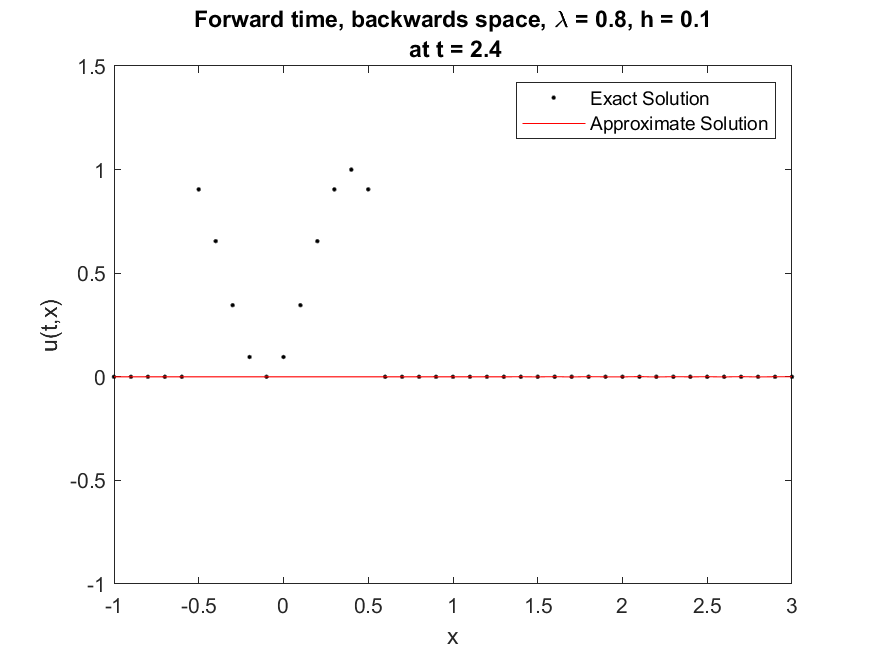
\includegraphics[width=.6\linewidth]{./code/a_forward_time_backward_space_h_one_10th.png}	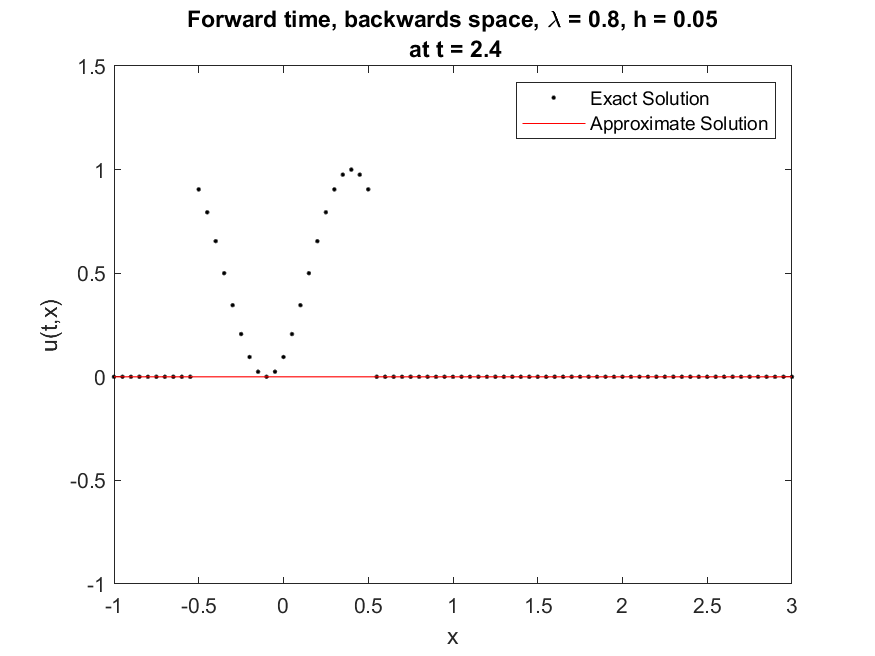
\includegraphics[width=.6\linewidth]{./code/a_forward_time_backward_space_h_one_20th.png}
	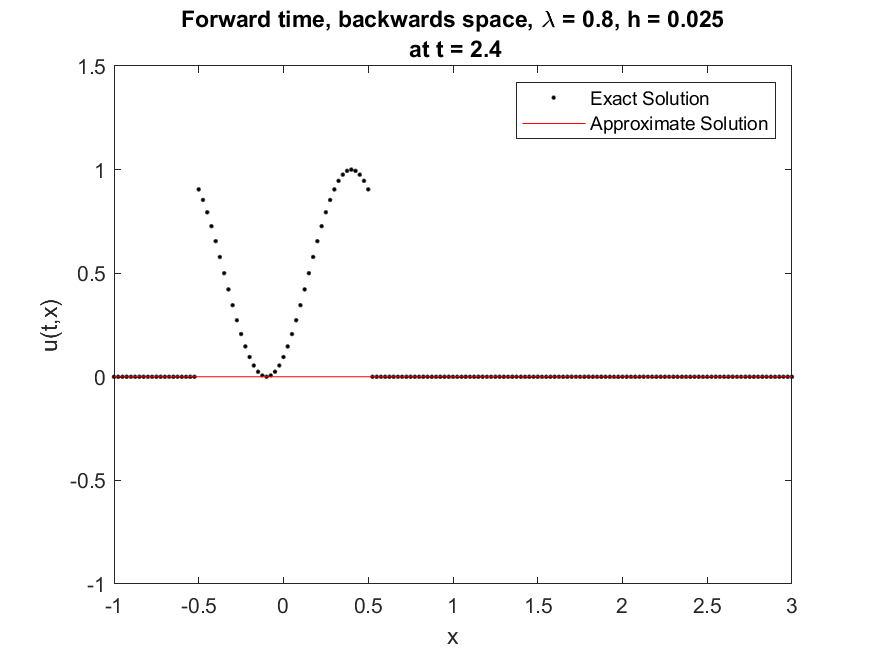
\includegraphics[width=.6\linewidth]{./code/a_forward_time_backward_space_h_one_40th.png}
	\caption{Forward time, backward space scheme at $t=2.4$ for $h-1/10, h=1/20$, and $h=1/40$, respectively}
\end{figure}

\subsubsection*{(b) Forward Time, Central Space}

Figure (2) shows this scheme. Notice that the approximate solution explodes to infinity  (see video, emailed). For $h=1/10$, the solution exceeds a value of 5 after about 1.76 seconds. For $h=1/20$, the solution exceeds 5 after about 1.2 seconds. For $h=1/40$, the solution passes 5 after about .72 seconds. As the density of the mesh doubles, the solution becomes useless more quickly.

\begin{figure}
	\centering
	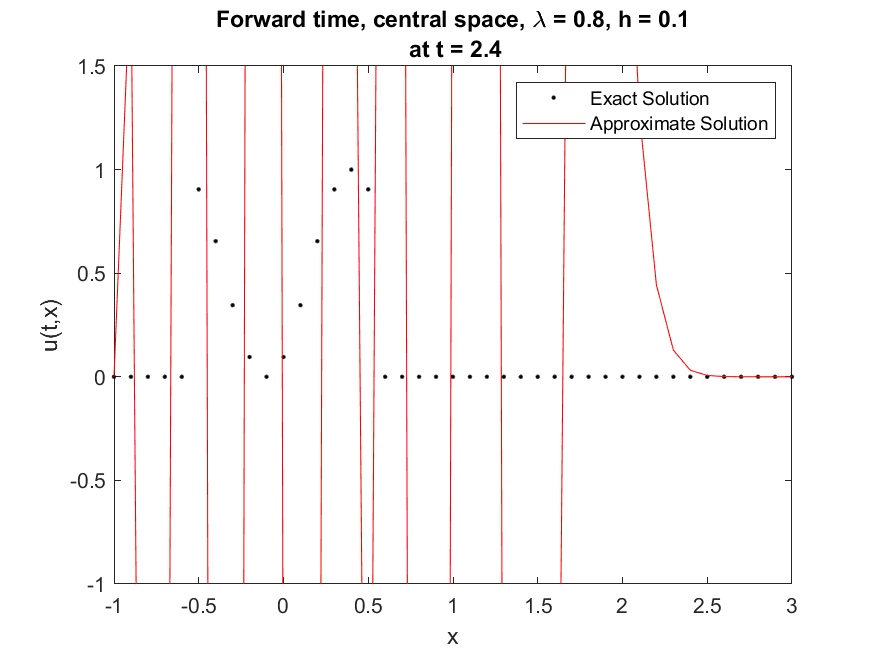
\includegraphics[width=.6\linewidth]{./code/b_forward_time_central_space_h_one_10th.png}	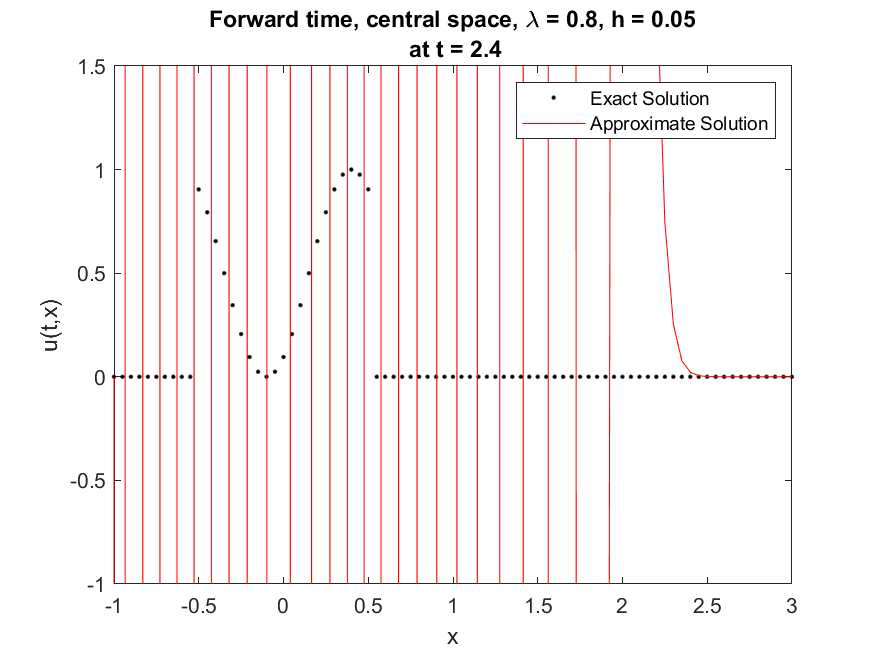
\includegraphics[width=.6\linewidth]{./code/b_forward_time_central_space_h_one_20th.png}
	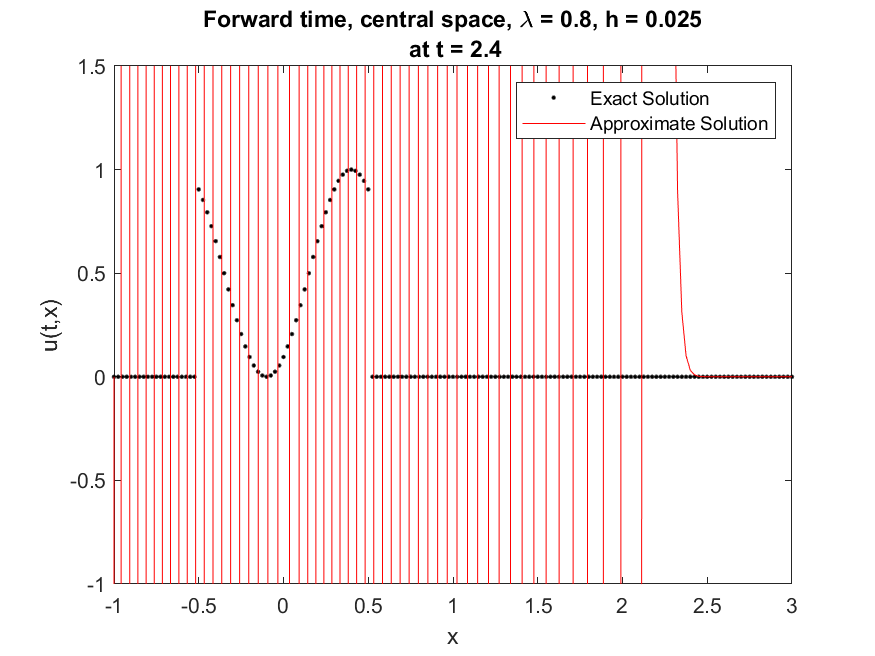
\includegraphics[width=.6\linewidth]{./code/b_forward_time_central_space_h_one_40th.png}
	\caption{Forward time, central space scheme at $t=2.4$ for $h-1/10, h=1/20$, and $h=1/40$, respectively}
\end{figure}

\subsubsection*{(c) Lax-Friedrichs}

Figure (3) shows this scheme. Notice that the approximate solution explodes to infinity (see video, emailed). For $h=1/10$, the solution exceeds a value of 5 after about 1.6 seconds. For $h=1/20$, the solution exceeds 5 after about 1.12 seconds. For $h=1/40$, the solution passes 5 after about .72 seconds. As the density of the mesh doubles, the solution becomes useless more quickly, in a similar scale to the forward time/central space scheme.

\begin{figure}
	\centering
	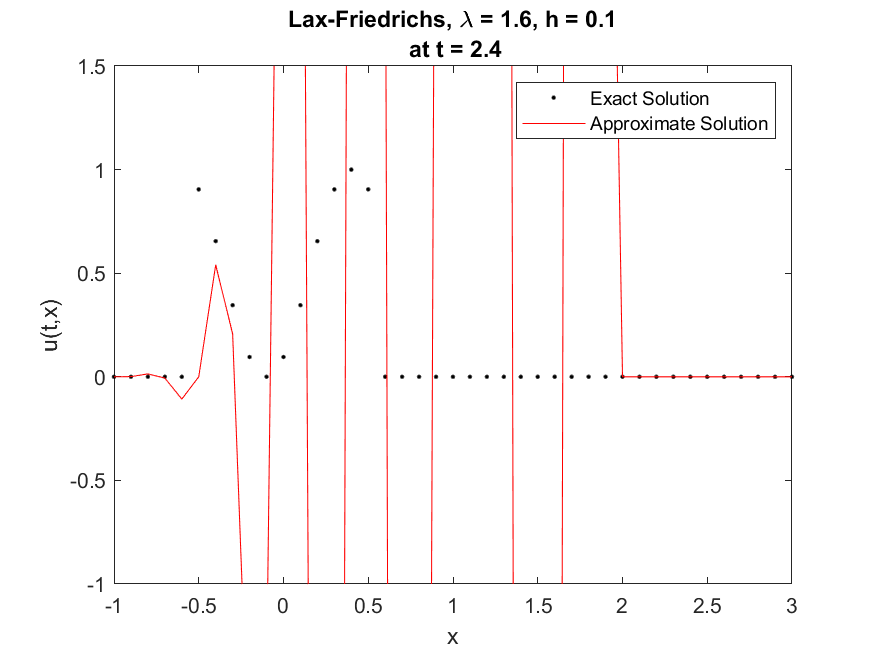
\includegraphics[width=.6\linewidth]{./code/c_lax_friedrichs_h_one_10th.png}	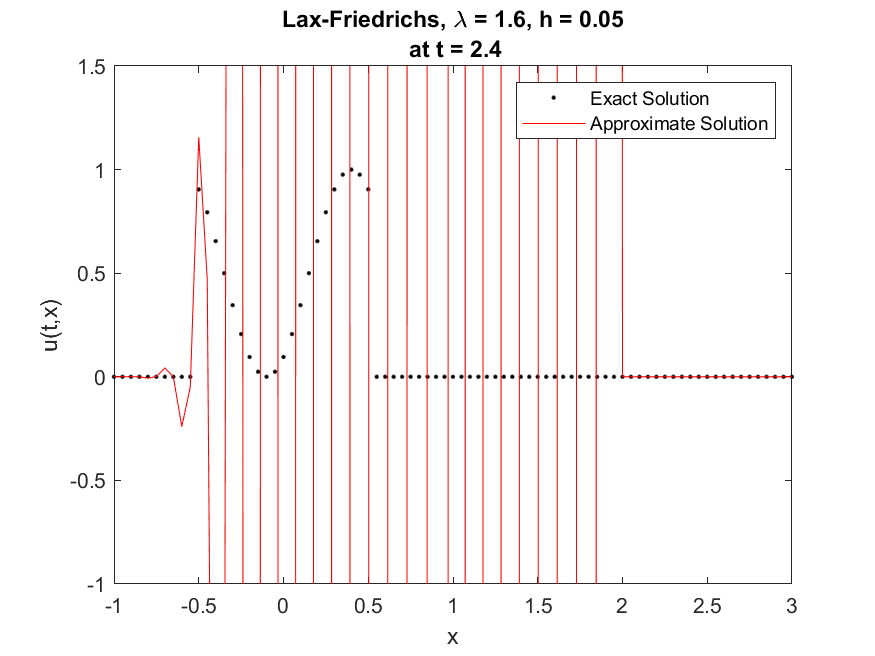
\includegraphics[width=.6\linewidth]{./code/c_lax_friedrichs_h_one_20th.png}
	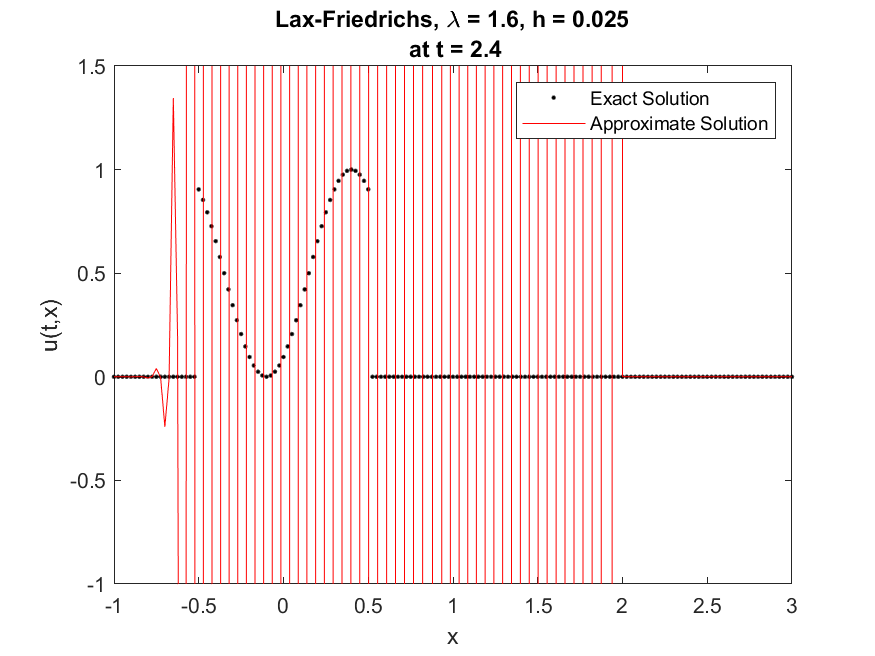
\includegraphics[width=.6\linewidth]{./code/c_lax_friedrichs_h_one_40th.png}
	\caption{Lax-Friedrichs at $t=2.4$ for $h-1/10, h=1/20$, and $h=1/40$, respectively}
\end{figure}

\subsubsection*{(d) Leapfrog}

Figure (4) shows this scheme. Notice that the approximate solution dampens to zero (see video, emailed). For $h=1/10$, it hits zero by about 0.72 seconds, like the forward time, backward space scheme. For $h=1/20$, it hits zero by about 0.36 seconds. For $h=1/40$, it hits zero by about 0.18 seconds. Just like (a), as the mesh density doubles, the time to convergence halves. Error? 

\begin{figure}
	\centering
	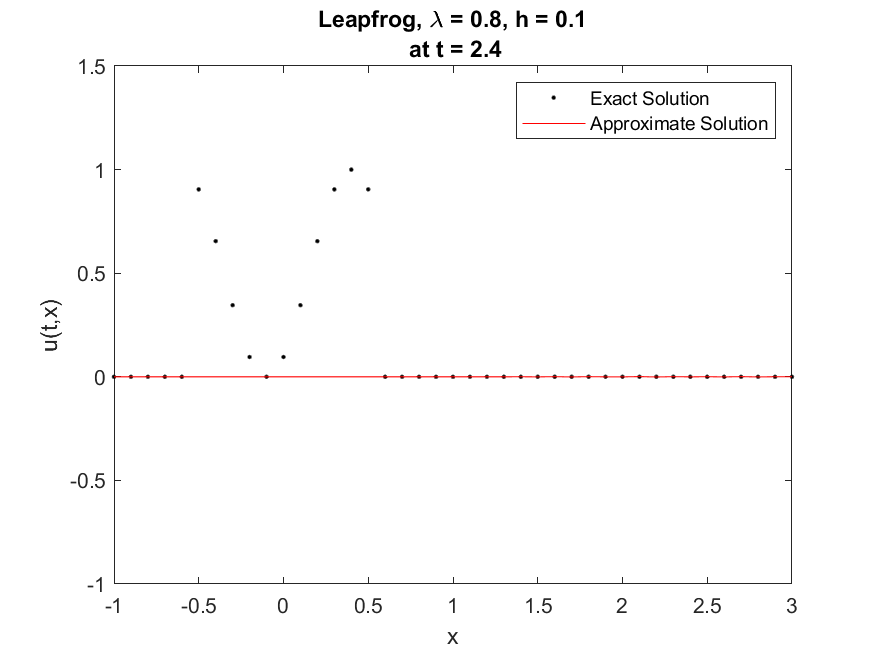
\includegraphics[width=.6\linewidth]{./code/d_leapfrog_h_one_10th.png}	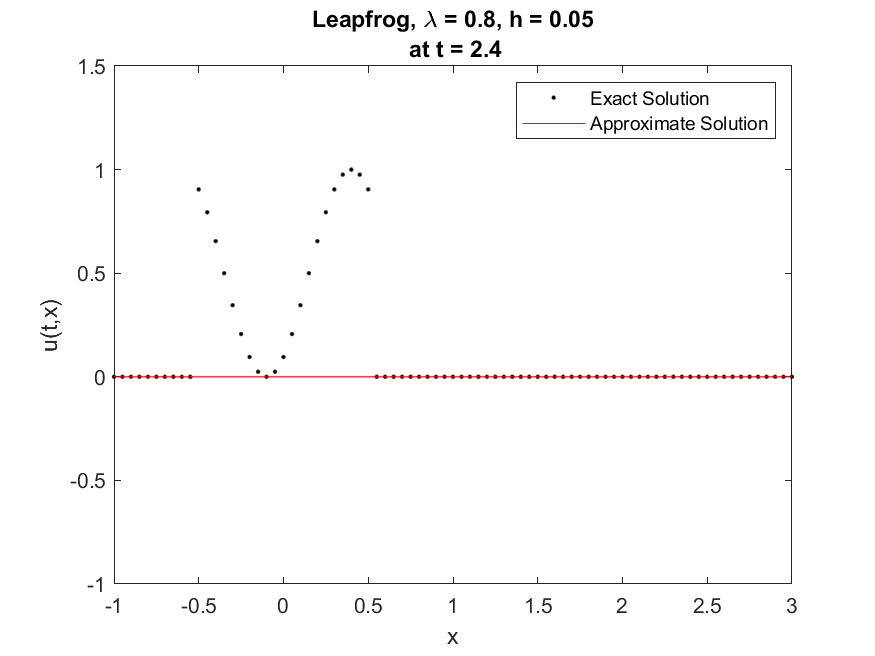
\includegraphics[width=.6\linewidth]{./code/d_leapfrog_h_one_20th.png}
	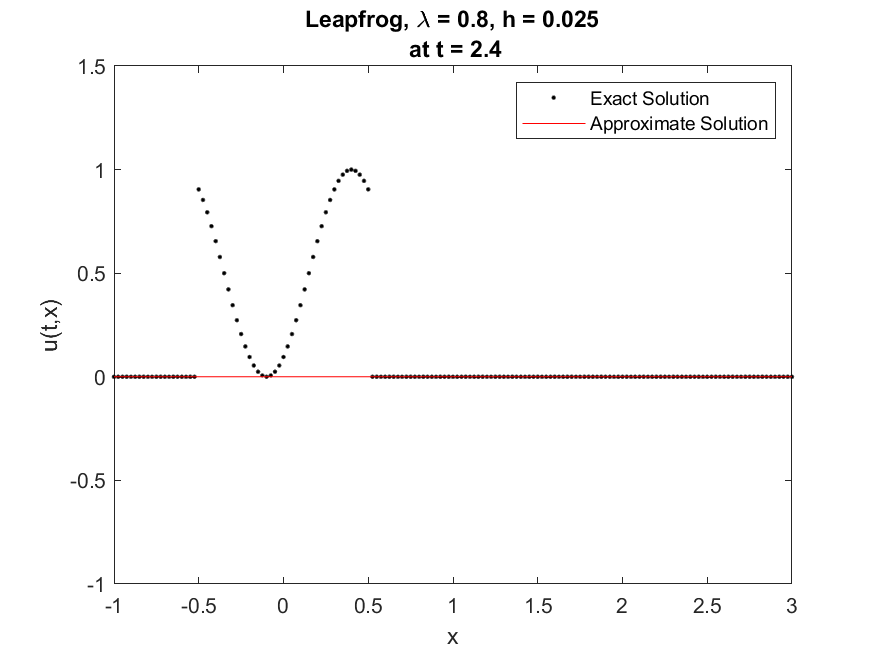
\includegraphics[width=.6\linewidth]{./code/d_leapfrog_h_one_40th.png}
	\caption{Forward time, backward space scheme at $t=2.4$ for $h-1/10, h=1/20$, and $h=1/40$, respectively}
\end{figure}

\section*{1.4.2}

Show that the leapfrog scheme is consistent with the one-way wave equation.

\subsubsection*{Solution}

\section*{1.5.1}

Show that schemes of the form
$$
u_{m}^{n+1}=\alpha u_{m+1}^{n}+\beta u_{m-1}^{n}
$$
are stable if $|\alpha|+|\beta|$ is less than or equal to 1. Conclude that the Lax-Friedrichs scheme is stable if $|a \lambda|$ is less than or equal to 1 .


\subsubsection*{Solution}

\section*{MATLAB Command Comments}


\end{document}









